\mode*
\lecture[app]{app}{app}

\section{Application Layer Protocols}

\subsection{HTTP}

\begin{frame}{\mode<beamer>{HTTP}}
  \mode<beamer>{ \includegraphics[width=\textwidth]{HTTP} }%
  \mode<article>{ \includegraphics[width=.5\textwidth]{HTTP} }
\end{frame}

\begin{frame}{HTTP Request (URL + Verb)}
  \begin{iblock}{URL}
    \centering
    \mode<beamer>{ \includegraphics[width=\textwidth]{Url} }%
    \mode<article>{ \includegraphics[width=.7\textwidth]{Url} }
  \end{iblock}
  \begin{center}
    \mode<beamer>{ 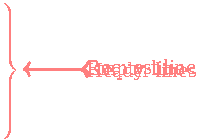
\includegraphics[width=.6\textwidth]{http-Req} }%
    \mode<article>{ 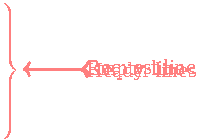
\includegraphics[width=.7\textwidth]{http-Req} }
  \end{center}
  \begin{iblock}{Verbs}
    \begin{tblr}{lllll}
      \textcolor{Green}{GET}&\textcolor{Red}{POST}&
      \textcolor{Red}{PUT}&\textcolor{Red}{PATCH}&\\
      \textcolor{Green}{HEAD}&\textcolor{Green}{OPTIONS}&
      \textcolor{Red}{DELETE}&\textcolor{Green}{TRACE}&CONNECT\\
    \end{tblr}
  \end{iblock}
\end{frame}

\begin{frame}{HTTP Response (Status Code + Message Body)}
  \centering
  \mode<beamer>{ 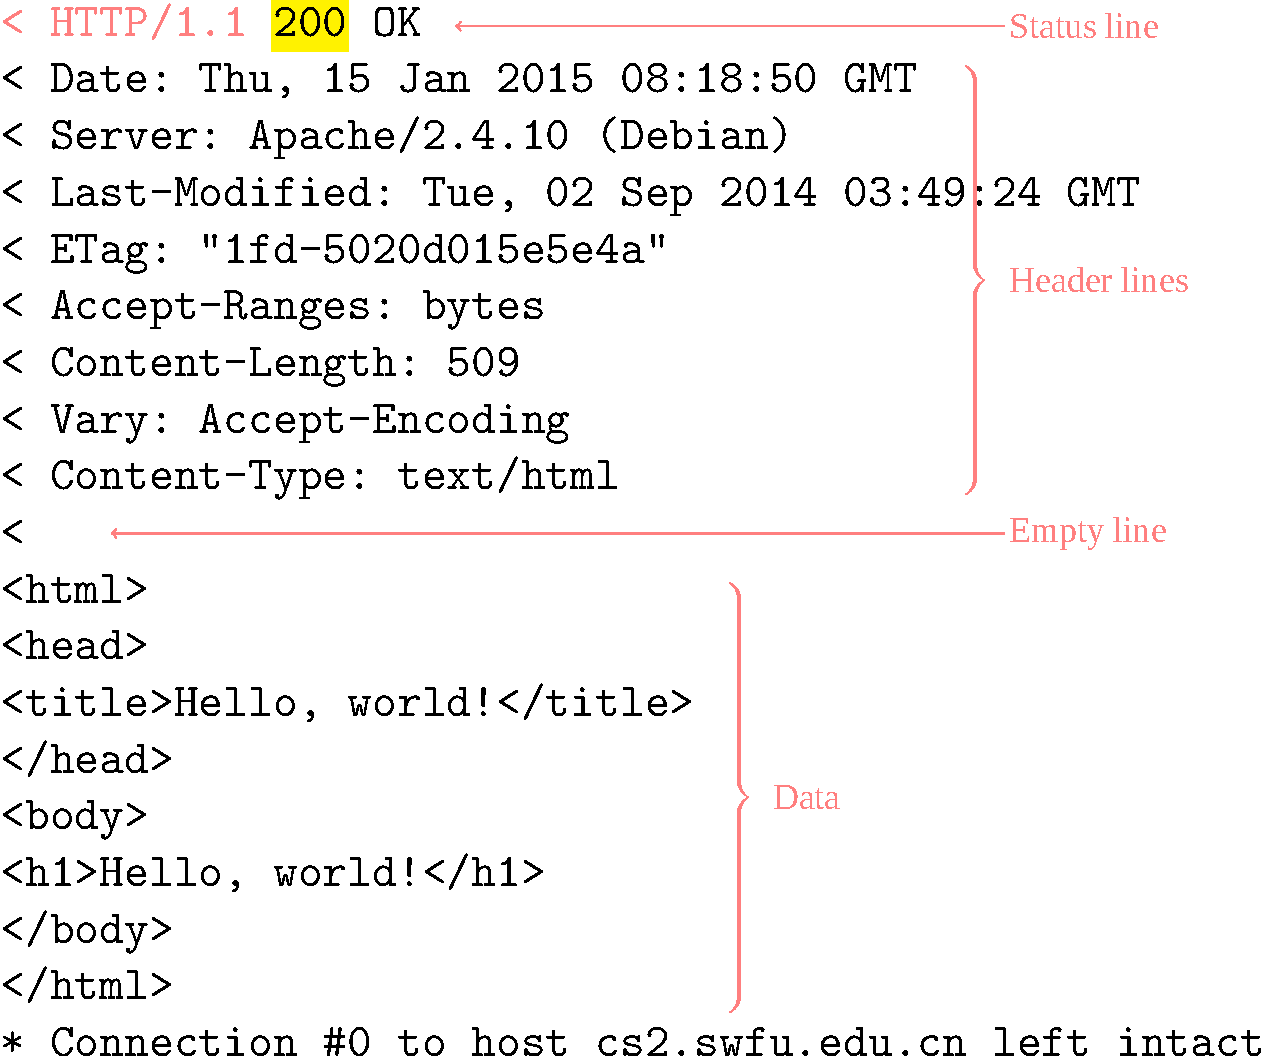
\includegraphics[height=.9\textheight]{http-Res} }%
  \mode<article>{ 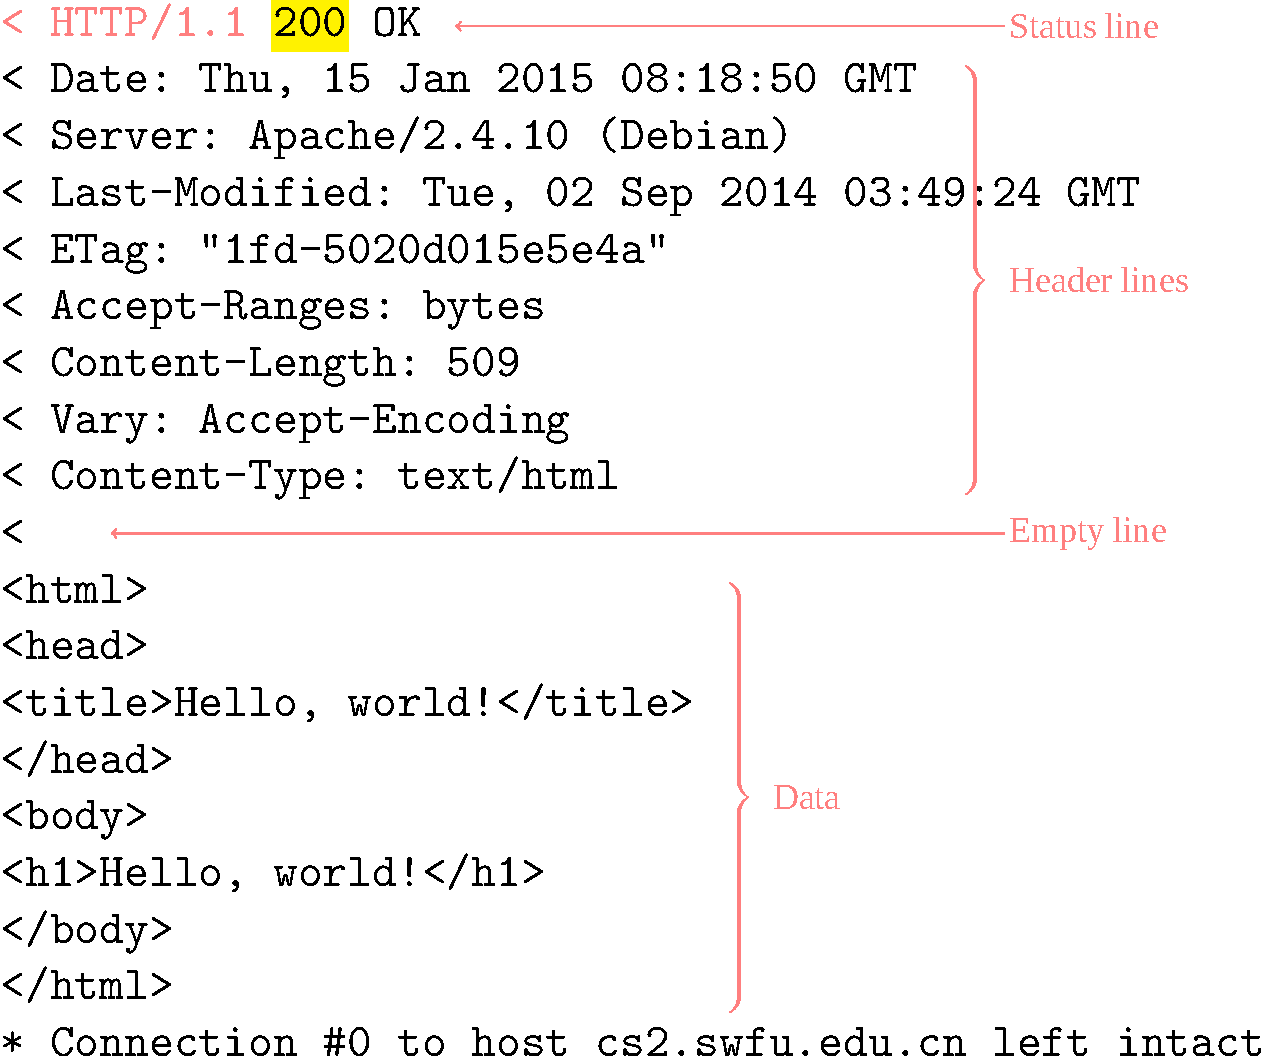
\includegraphics[width=.5\textwidth]{http-Res} }
\end{frame}

\begin{frame}{Status Codes}
  \begin{description}
  \item[1xx] Informational Messages
    \begin{itemize}
    \item[e.g.] \texttt{104 Connection Reset by Peer}
    \end{itemize}
  \item[2xx] Successful
    \begin{itemize}
    \item[e.g.] \texttt{200 OK}
    \end{itemize}
  \item[3xx] Redirection
    \begin{itemize}
    \item[e.g.] \texttt{301 Moved Permanently}
    \end{itemize}
  \item[4xx] Client Error
    \begin{itemize}
    \item[e.g.] \texttt{404 Not Found}
    \end{itemize}
  \item[5xx] Server Error
    \begin{itemize}
    \item[e.g.] \texttt{500 Internal Server Error}
    \end{itemize}
  \end{description}
  % \href{http://tools.ietf.org/html/rfc2616\#section-6.1.1}{RFC2616, Sec 6.1.1}
\end{frame}

\begin{frame}{HTTP Transaction}
  \begin{iblock}{Non-persistent --- separate TCP connection}
    \begin{center}
      \mode<beamer>{ 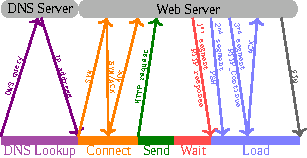
\includegraphics[width=.8\textwidth]{http-transaction} }%
      \mode<article>{ 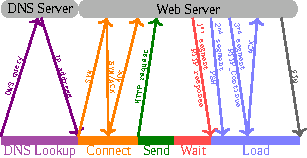
\includegraphics[width=.5\textwidth]{http-transaction} }
    \end{center}
  \end{iblock}
\end{frame}

\begin{frame}
  \begin{iblock}{Persistent --- same TCP connection}
    \begin{center}
      \mode<beamer>{ 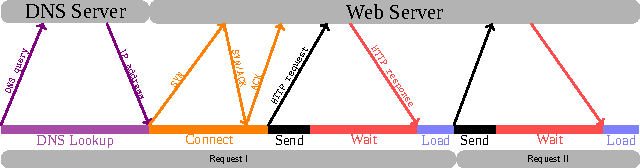
\includegraphics[width=\textwidth]{persistent-transaction} }%
      \mode<article>{ 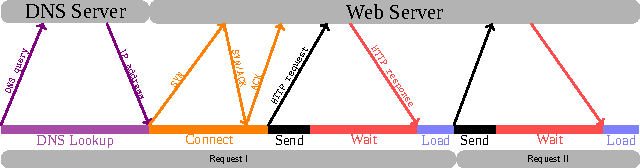
\includegraphics[width=.7\textwidth]{persistent-transaction} }
    \end{center}
  \end{iblock}
\end{frame}

\href{http://blog.catchpoint.com/2010/09/17/anatomyhttp/}{Anatomy of an HTTP Transaction}

\begin{frame}{Stateless Protocol}
  \begin{minipage}{.35\linewidth}
    A HTTP server maintains no information about the clients.
    \begin{itemize}
    \item[☺] Simplifies server design
    \item[☺] Save server resources
    \item[☺] Serve more users
    \item[\alert{☹}] Missing information
    \end{itemize}
  \end{minipage}\hfill
  \begin{minipage}{.6\linewidth}
    Keeping user state with cookies
    
    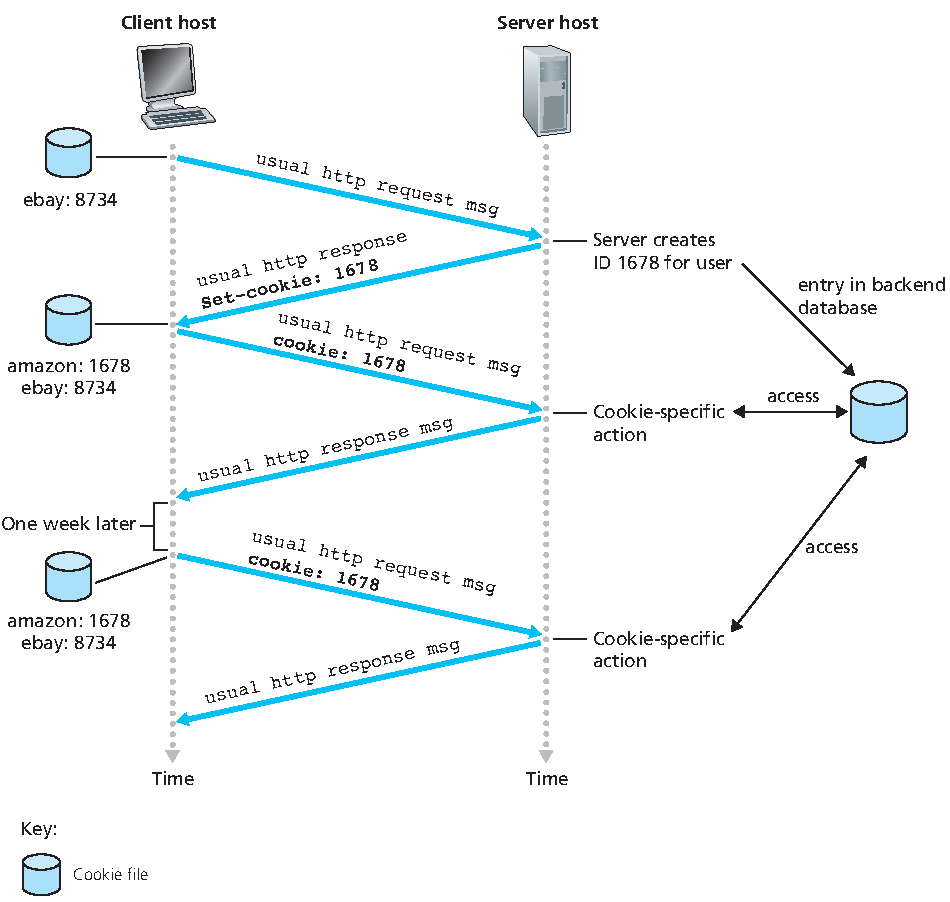
\includegraphics[width=1.1\textwidth]{cookie}
  \end{minipage}  
\end{frame}

See also \citetitle[Sec.~2.2.4, \emph{User-Server Interaction: Cookies}]{kurose2013computer}

\begin{frame}{HTTP/2}
  \begin{iblock}{Quoted from \url{http://http2.github.io/faq/}}
    \begin{itemize}
    \item is binary, instead of textual
    \item is fully multiplexed, instead of ordered and blocking
    \item can therefore use one connection for parallelism
    \item uses header compression to reduce overhead
    \item allows servers to “push” responses proactively into client caches
    \end{itemize}
  \end{iblock}
  \begin{description}
  \item[May 2015] Publish HTTP/2 as RFC7540/7541
  \end{description}
\end{frame}

See also:
\begin{itemize}
\item \url{http://en.wikipedia.org/wiki/HTTP/2}
\item \url{http://http2.github.io/faq/}
\item \url{https://bagder.gitbooks.io/http2-explained/en}
\end{itemize}

\begin{frame}[fragile]{HTML}
  \begin{minted}[fontsize=\small,
    linenos=true,numbersep=10pt,
    frame=leftline,framesep=3pt,rulecolor=\color{lightgray},
    xleftmargin=1cm,xrightmargin=1cm,
    % gobble=4
    ]{html}
<html>
    <head>
        <title>Hello, world!</title>
    </head>
    <body>
        <H1>Hello, world!</H1>
    </body>
</html>
  \end{minted}
\end{frame}

\begin{frame}{
\includegraphics[height=2em]{lamp-logo}}
  \centering
  \mode<beamer>{ 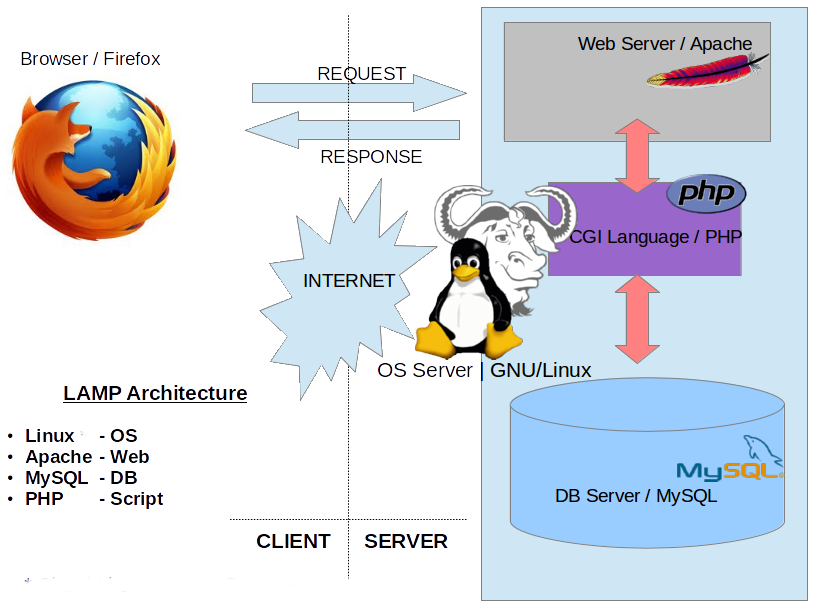
\includegraphics[height=.9\textheight]{lamp} }%
  \mode<article>{ 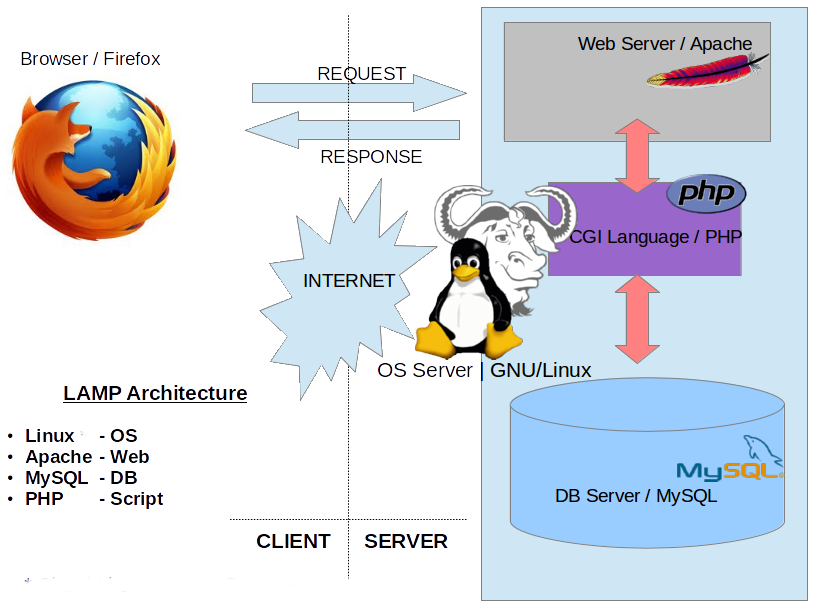
\includegraphics[width=.5\textwidth]{lamp} }
\end{frame}

Questions:
\begin{enumerate}
\item What about HTTP over UDP?
\end{enumerate}

\begin{frame}[allowframebreaks]{HTTP References}
  \begin{refsection}
    \nocite{wiki:http, wiki:httptwo, wiki:cookie, wiki:stateless, wiki:html, wiki:lamp,
      rfc2616, rfc7540, rfc7541}
    \printbibliography[heading=none]
  \end{refsection}
\end{frame}

%\mode<article>{\clearpage}
\subsection{DNS}

\begin{frame}\mode<beamer>{\frametitle{DNS}}\framesubtitle{Names and Addresses}
  \begin{iblock}{RFC 791, page 7:}
    \begin{description}
    \item[A name] indicates what we seek
    \item[An address] indicates where it is
    \item[A route] indicates how to get there
    \end{description}
  \end{iblock}
  \begin{itemize}
  \item A name (hostname) can be assigned to any device that has an IP address.
  \item The network software doesn't require names, but they do make it easier for humans
    to use the network.
  \end{itemize}
\end{frame}

\begin{frame}{The DNS Name Space Is Hierarchical}
  \begin{iblock}{The domain hierarchy is similar to the UNIX filesystem}
    \begin{center}
      \mode<beamer>{ \includegraphics[width=\textwidth]{dns_tree} }%
      \mode<article>{ \includegraphics[width=.8\textwidth]{dns_tree} }
    \end{center}\label{fig:dns_tree}
  \end{iblock}
  \begin{itemize}
  \item Organizational: \texttt{com}, \texttt{edu}, \texttt{gov}, \texttt{mil}, \texttt{net},
    \texttt{org}, \texttt{int}
  \item Geographic: \texttt{cn}, \texttt{us}, \texttt{uk}, \texttt{jp}, \texttt{de}, etc.
  \end{itemize}
\end{frame}

\begin{frame}
  \begin{itemize}
  \item[\$] \texttt{ssh someone@cs3.swfu.edu.cn}
  \end{itemize}
  \begin{minipage}{.5\linewidth}
    \begin{iblock}{}
      \mode<beamer>{ 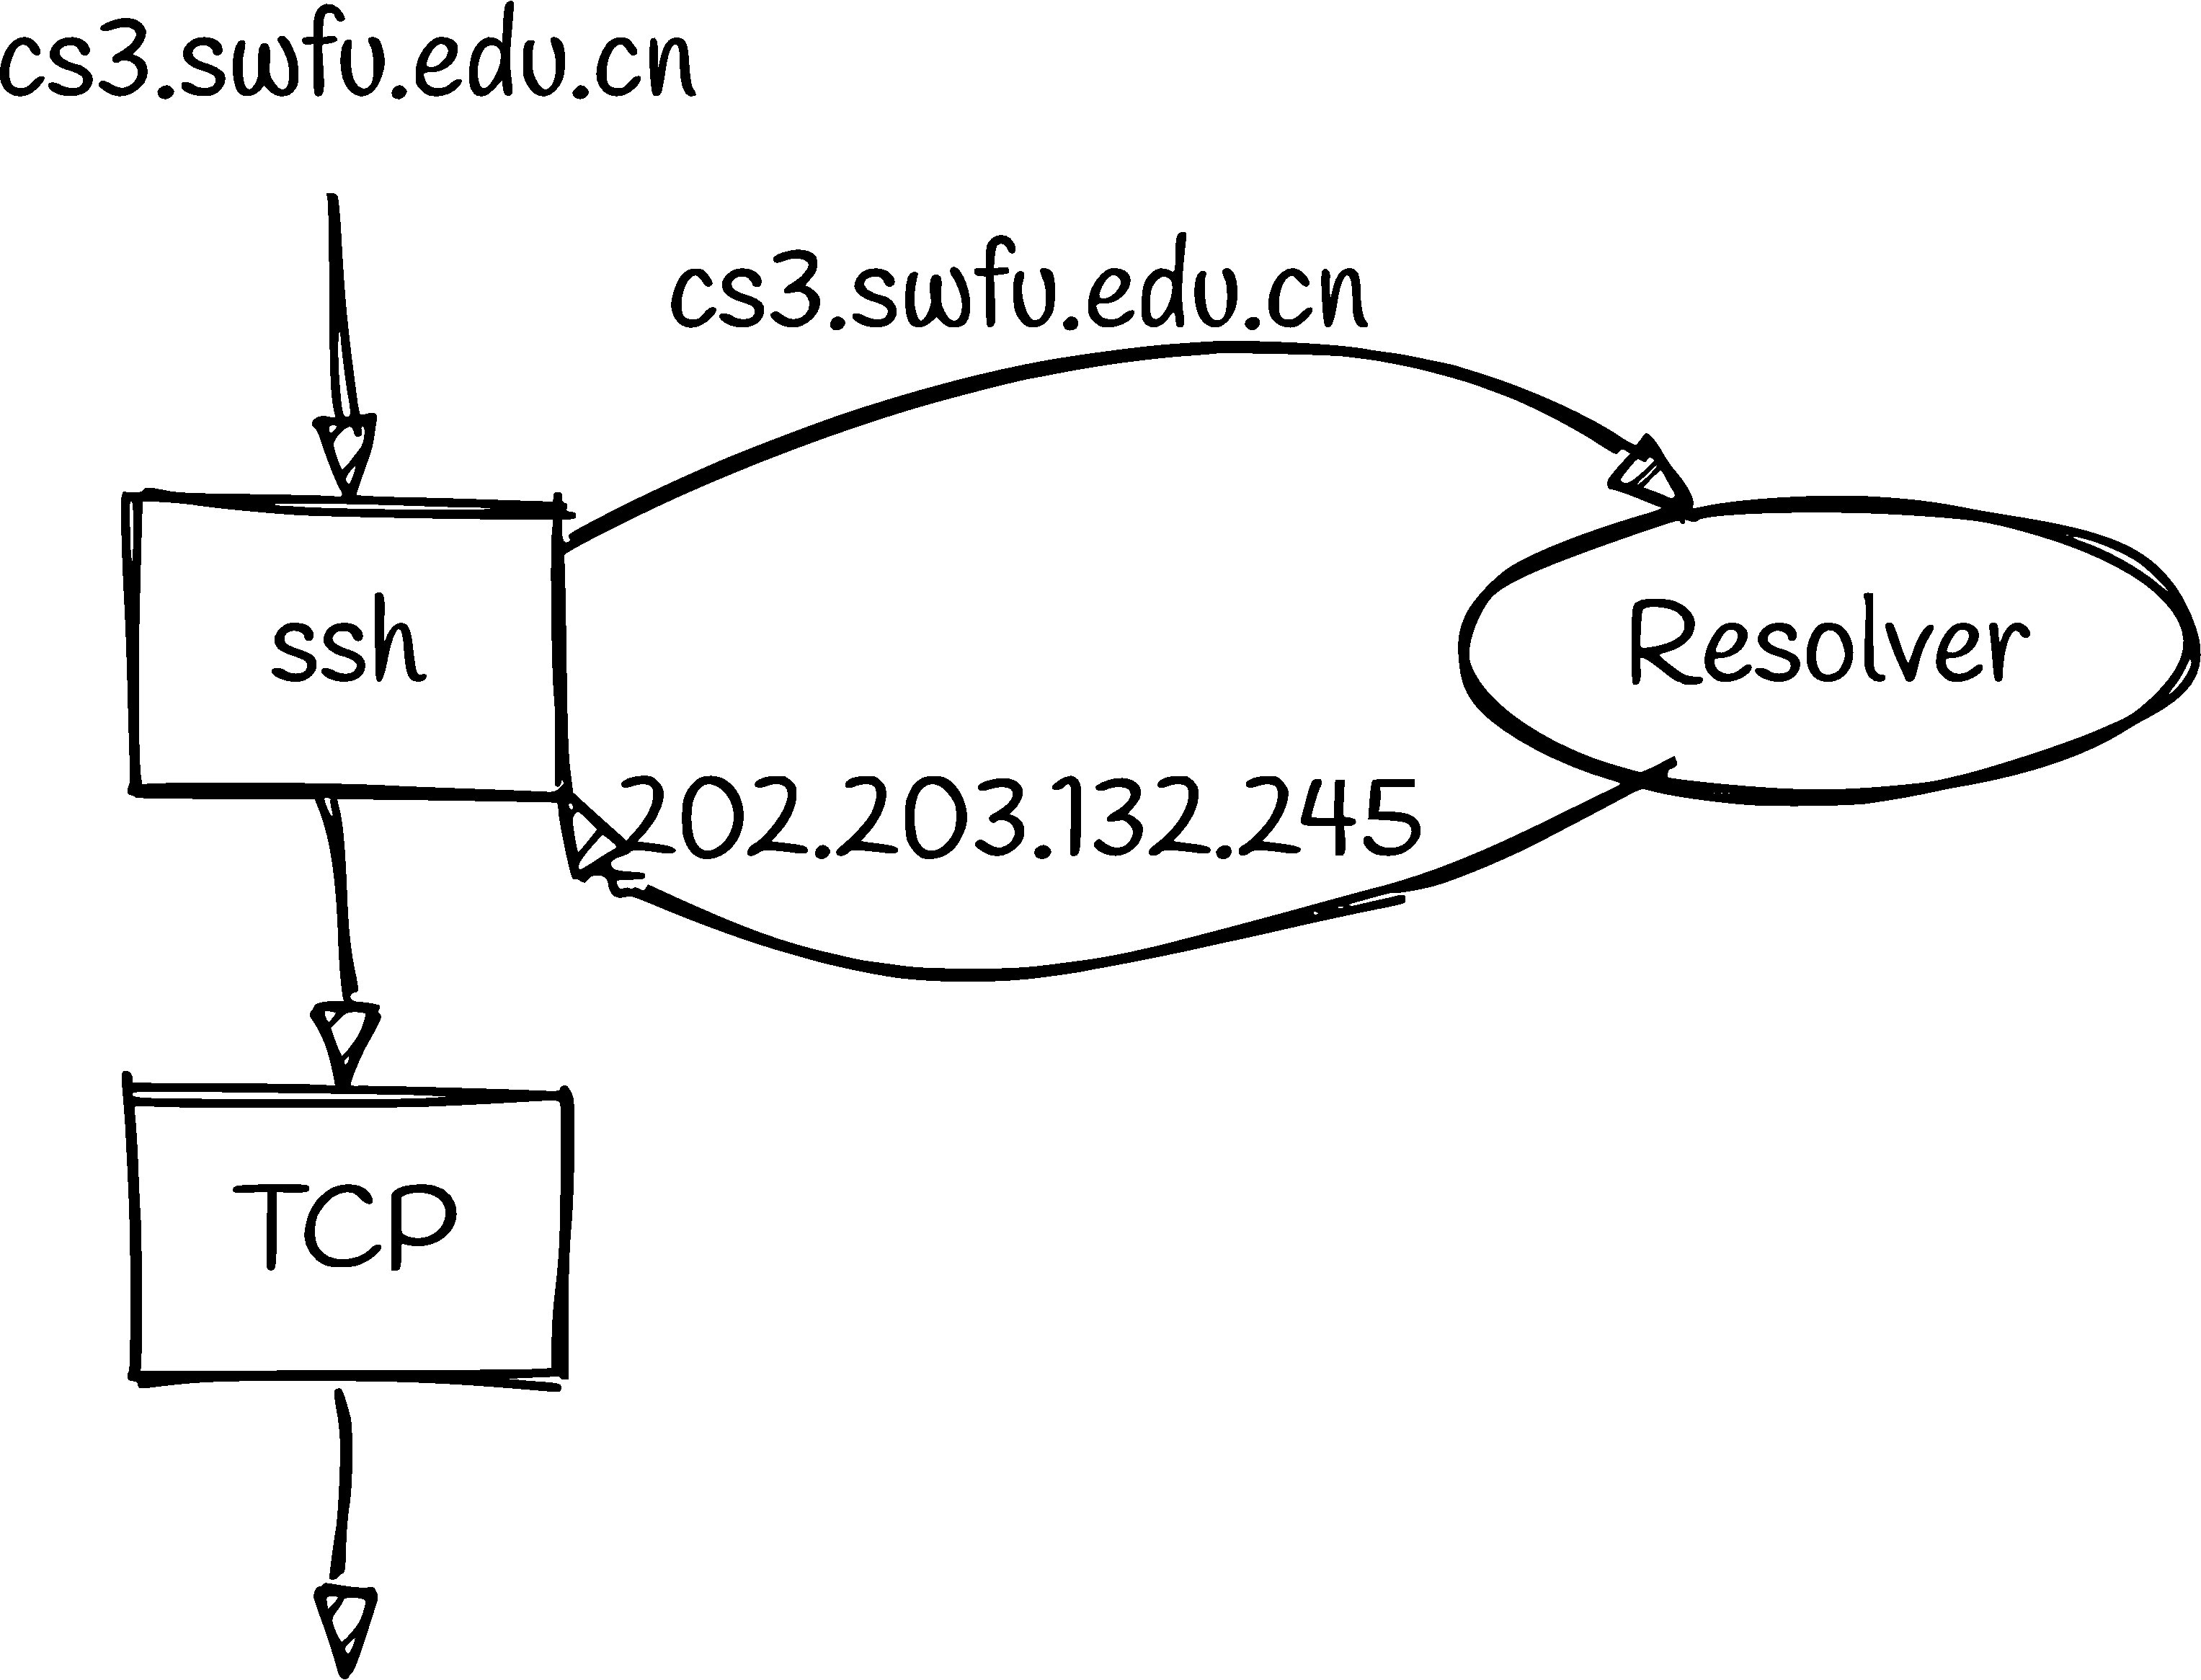
\includegraphics[width=\textwidth]{resolver} }%
      \mode<article>{ 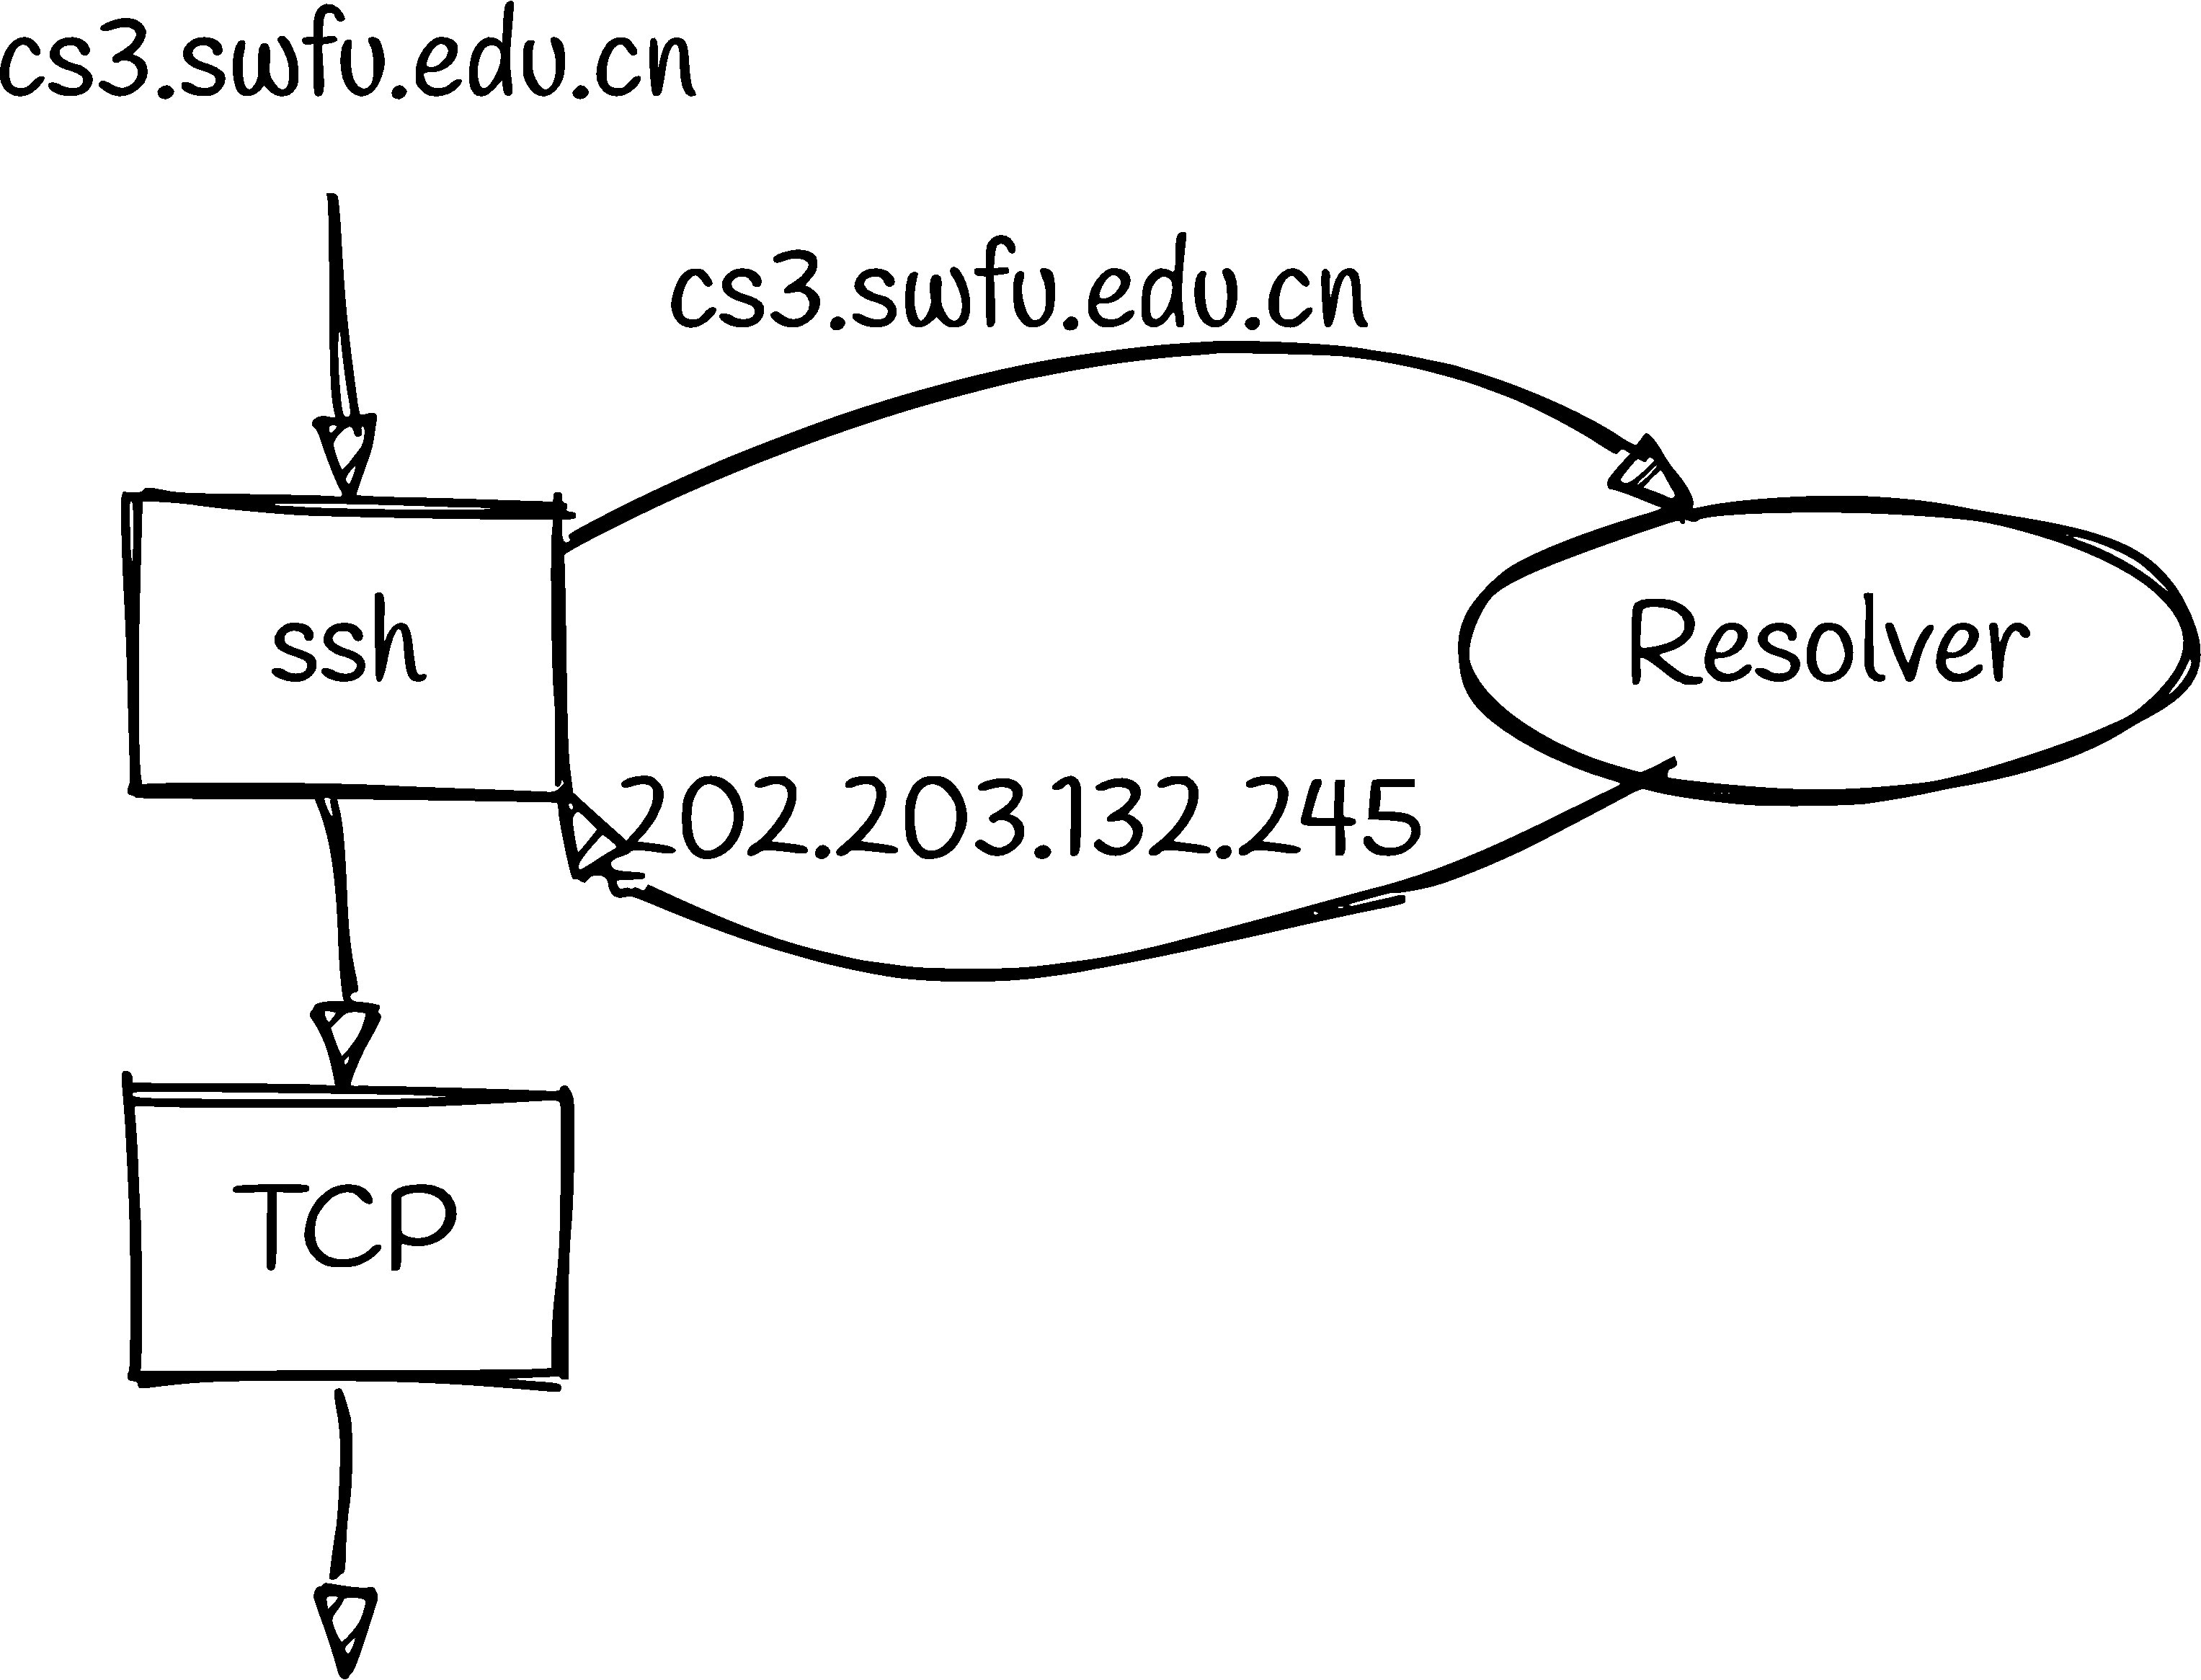
\includegraphics[width=\textwidth]{resolver} }
    \end{iblock}
  \end{minipage}
  \begin{minipage}{.45\linewidth}
    \begin{itemize}
    \item Resolver is normally part of the application
      \begin{itemize}
      \item \texttt{man 3 gethostbyname}
      \item \texttt{man 3 gethostbyaddr}
      \end{itemize}
    \item The TCP/IP protocols within the kernel know nothing about the DNS
    \end{itemize}
  \end{minipage}
\end{frame}

\begin{frame}{Typical Configuration}
  \begin{center}
    \mode<beamer>{
      \includegraphics[width=\textwidth]{dns-typical}
    } \mode<article>{
      \includegraphics[width=.5\textwidth]{dns-typical}
    }
  \end{center}
\end{frame}

\begin{frame}{Translating Names Into Addresses}
  Two common ways:
  \begin{description}
  \item[Host table] The old way --- \texttt{/etc/hosts}
  \item[DNS] A distributed database system --- Domain Name Service (DNS)
  \end{description}
\end{frame}

\begin{frame}{The Host Table --- \texttt{/etc/hosts}}
  \begin{center}\ttfamily
    \begin{tblr}{colspec={lll}%,row{even}={gray9}
      }
      127.0.0.1       & localhost &                 \\
      39.129.9.40     & cs6       & cs6.swfu.edu.cn \\
      202.203.132.245 & cs3       & cs3.swfu.edu.cn \\
      202.203.132.242 & cs2       & cs2.swfu.edu.cn
    \end{tblr}
  \end{center}
  It's still widely used, because:
  \begin{itemize}
  \item The important hosts on the local network
  \item NIS host database
  \item Local intranet
  \item In case DNS is not running
  \end{itemize}
\end{frame}

See also \citetitle[\emph{RFC 952}]{rfc952}

\begin{frame}{All hosts connected to the Internet should use DNS}
  \begin{iblock}{The old host table system is inadequate for the global Internet}
    \begin{enumerate}
    \item[\alert{☹}] Inability to scale
    \item[\alert{☹}] Lack of an automated update process.
    \end{enumerate}

    \begin{description}
    \item[Old story] Prior to adopting DNS, the Network Information Center (NIC)
      maintained a large table of Internet hosts called the NIC host table. Hosts included
      in the table were called registered hosts, and the NIC placed hostnames and
      addresses into this file for all sites on the Internet.
    \end{description}    
  \end{iblock}
\end{frame}

\begin{frame}{Domain Name System (DNS)}
  \begin{itemize}
  \item Scales well
    \begin{itemize}
    \item Doesn't rely on a single large table
    \item Distributed database system that doesn't bog down as the database grows
    \end{itemize}
    DNS currently provides information on approximately 16,000,000 hosts, while less than
    10,000 are listed in the host table.
  \item Guarantees that new host information will be disseminated to the rest of the
    network as it is needed
  \end{itemize}
\end{frame}

\begin{frame}{DNS softwares}
  \begin{center}
    \mode<beamer>{ \includegraphics[width=.7\textwidth]{dns-sw} }%
    \mode<article>{ \includegraphics[width=.3\textwidth]{dns-sw} }
  \end{center}
  \begin{description}
  \item[The resolver]  asks the questions.
  \item[The name server]  answers the questions.
  \end{description}
\end{frame}

\begin{frame}{Example: \emph{sale.plant.nuts.com?}}
  \begin{iblock}{Recursive query}    
    \begin{center}
      \includegraphics[width=\textwidth]{dns-recur}
    \end{center}
  \end{iblock}
  \begin{iblock}{Non-recursive query}
    The remote server tells the local server who to ask next
    \begin{center}
      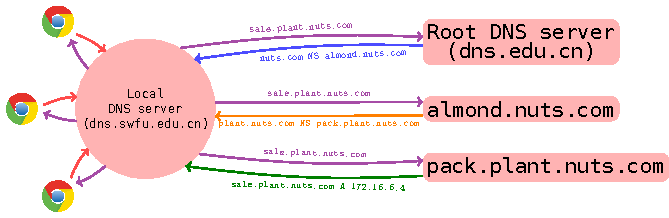
\includegraphics[width=.8\textwidth]{dns-nonrecur}\label{fig:non_recursive}
    \end{center}
  \end{iblock}
\end{frame}

% \begin{frame}{Name Servers}
%   \begin{iblock}{The three main categories of name servers are:}
%     \begin{description}
%     \item[Primary server:] gets its information from a disk file
%       \begin{itemize}
%         % \item It loads the domain's information directly from a disk
%         %   file created by the domain administrator.
%       \item It has complete information about its domain and its response is always
%         accurate.
%       \end{itemize}
%       % There should be only one primary server for a domain.
%     \item[Secondary server:] obtains all the information from the primary
%       \begin{itemize}
%       \item It's a backup server
%       \end{itemize}
%       % a backup nameserver to relieve traffic
%       % on the main server and to have an alternative source for
%       % information when your primary nameserver is unavailable.
%     \item[Caching-only server:] it just remembers the answers to previous lookups in case
%       the same lookup is performed again.
%     \end{description}
%   \end{iblock}
% \end{frame}

% \begin{frame}
%   \begin{iblock}{With DNS, information is automatically disseminated, and only to those who
%       are interested.}
%     \begin{itemize}
%     \item If a DNS server receives a request for information about a host for which it has
%       no information, it passes on the request to an \emph{authoritative server}.
%       \begin{description}
%       \item[An authoritative server] is any server responsible for maintaining accurate
%         information about the domain being queried.
%       \end{description}
%     \item When the authoritative server answers, the local server saves (caches) the
%       answer for future use.
%     \item The next time the local server receives a request for this information, it
%       answers the request itself.
%     \end{itemize}
%   \end{iblock}
% \end{frame}

\begin{frame}{Resource Records}
  \begin{minipage}{.25\linewidth}
    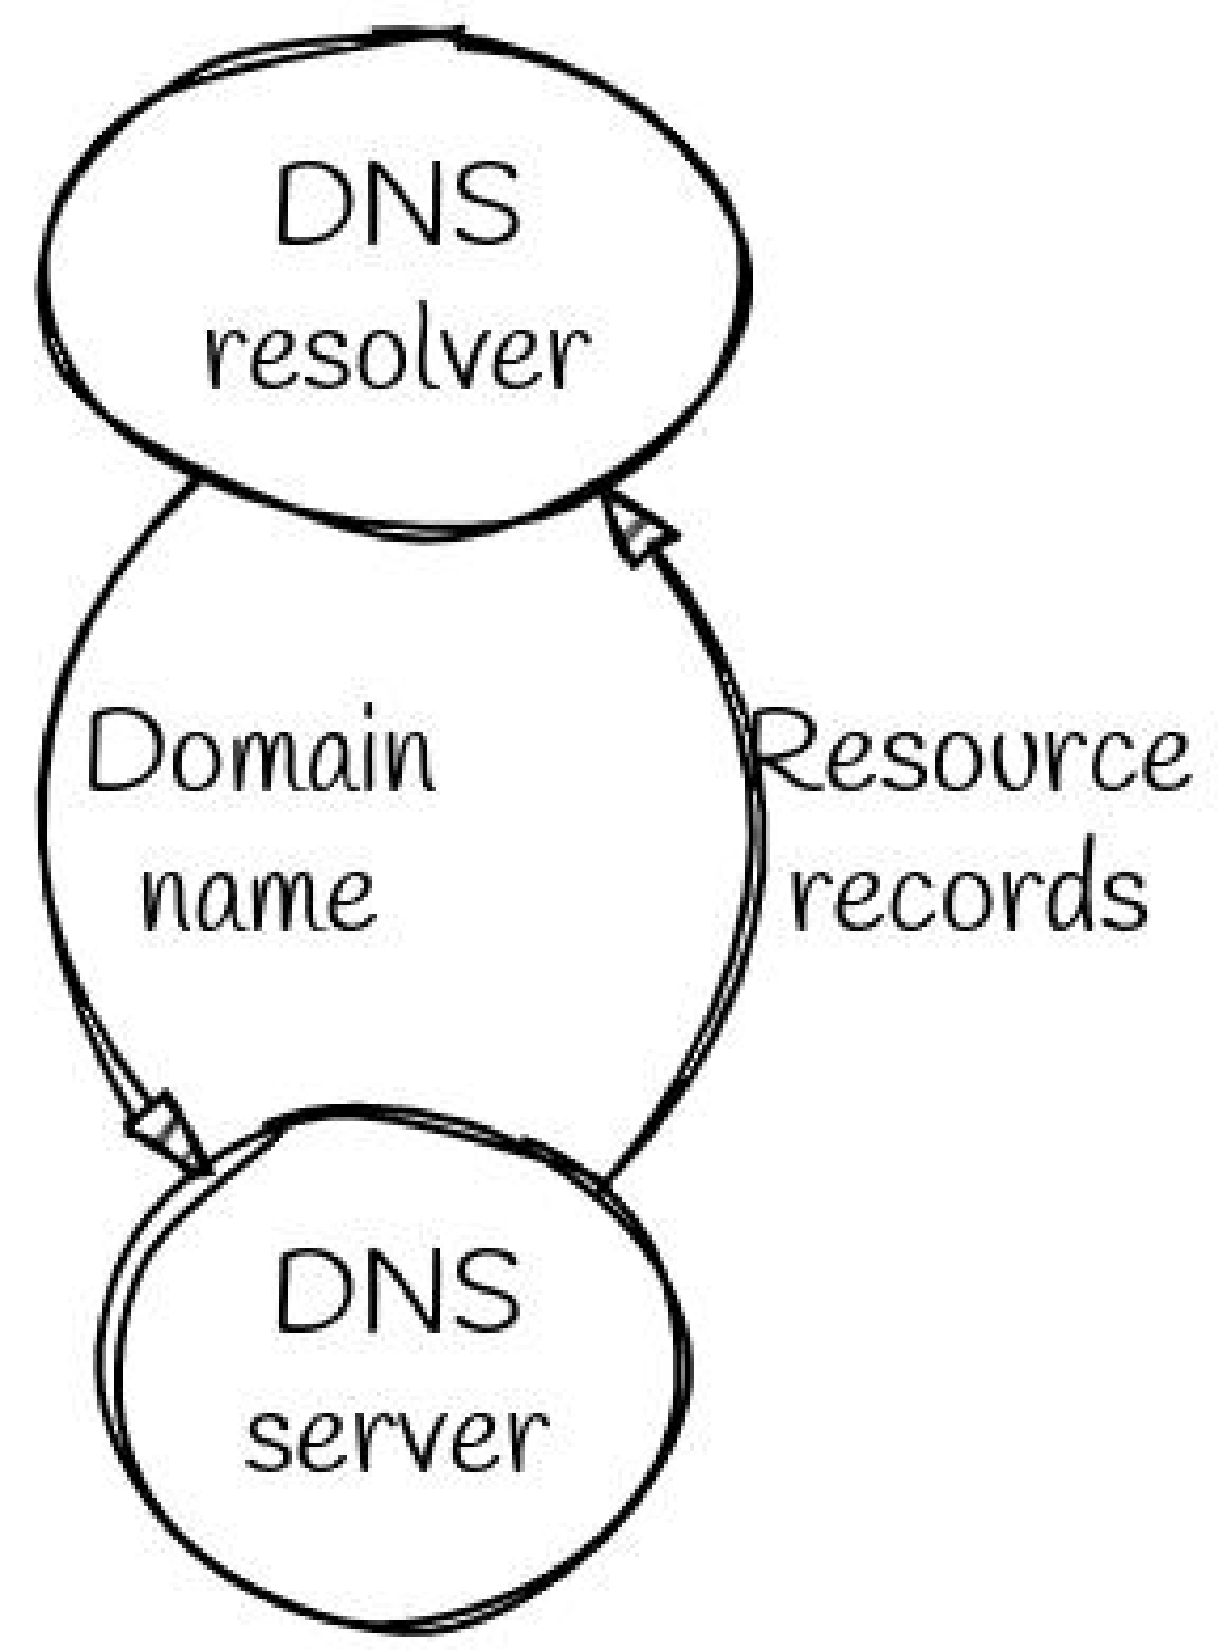
\includegraphics[width=\textwidth]{dns-sw2}
  \end{minipage}
  \begin{minipage}{.7\linewidth}
    \begin{iblock}{What's associated with a domain name?}
      \begin{small}
        \begin{tblr}{%
            colspec={lll}, row{odd}={gray9},%
            column{1}={font=\ttfamily},row{1}={font=\bfseries}}
          Type  & Meaning              & Value                            \\
          A     & IP address of a host & 32-bit integer                   \\
          NS    & Name Server          & Name of a server for this domain \\
          MX    & Mail eXchange        & Domain willing to accept email   \\
          HINFO & Host INFOrmation     & CPU and OS in ASCII              \\
          CNAME & Canonical NAME       & Domain name                      \\
          PTR   & PoinTeR              & Alias for an IP address          \\
          % TXT & TeXT                 & Uninterpreted ASCII text         \\
          % SOA & Start of Authority   & Parameters for this zone         \\
        \end{tblr}
      \end{small}
    \end{iblock}
  \end{minipage}
  % When a resolver gives a domain name to DNS, what it gets back are the \emph{resource
  % records} associated with that name.
\end{frame}

See also: \citetitle[Sec.~4, \emph{Messages}]{rfc1035}

\begin{frame}{Resource Records Example}
  \centering
  \mode<beamer>{ \includegraphics[height=.9\textheight]{dns-rr2} }%
  \mode<article>{ \includegraphics[width=.6\textwidth]{dns-rr2} }
\end{frame}

\begin{frame}{DNS Message Format}
  \begin{center}
    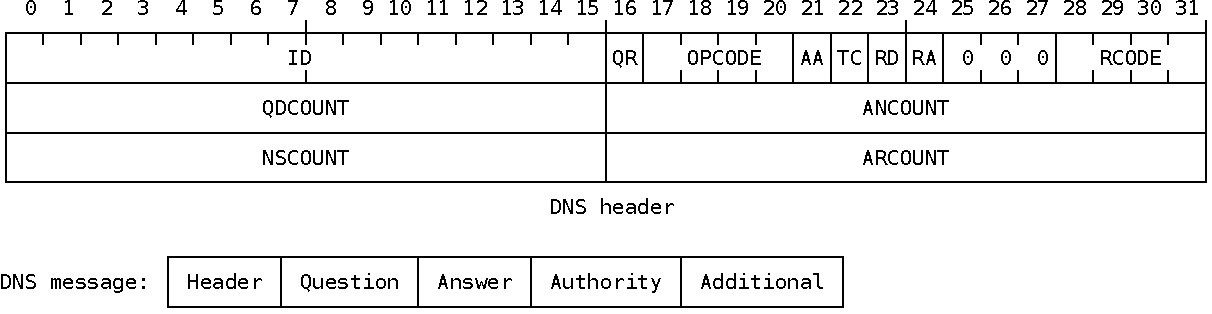
\includegraphics[width=\textwidth]{dns-hdr}
  \end{center}

  \begin{multicols}{2}{\scriptsize 
      \begin{description}
      \item[QR:] Query/Response
        \begin{itemize}
        \item[0:] {\scriptsize query}
        \item[1:] {\scriptsize response}
        \end{itemize}
      \item[OPCODE:] operation type
        \begin{itemize}
        \item[0:] {\scriptsize a standard query}
        \item[1:] {\scriptsize an inverse query}
        \item[2:] {\scriptsize server status request}
        \end{itemize}
      \item[AA:] authoritative answer
      \item[TC:] truncated. only the first 512 bytes of reply was returned
      \item[RD:] Recursion Desired
      \item[RA:] Recursion Available
      \item[RCODE:] return code. common values:
        \begin{itemize}
        \item[0:] {\scriptsize no error}
        \item[3:] {\scriptsize name error}
        \end{itemize}
      \end{description}}
\end{multicols}
\end{frame}

\begin{frame}
  \begin{center}
    \mode<beamer>{ 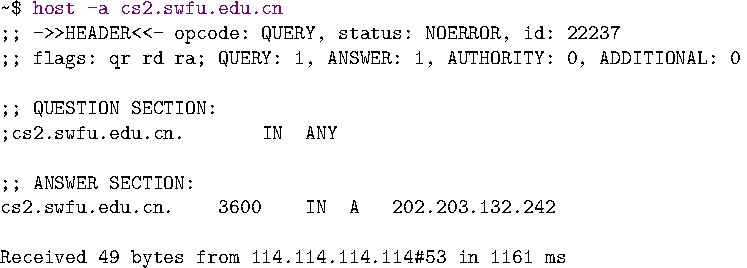
\includegraphics[width=\textwidth]{dns-rr-swfu} }%
    \mode<article>{ 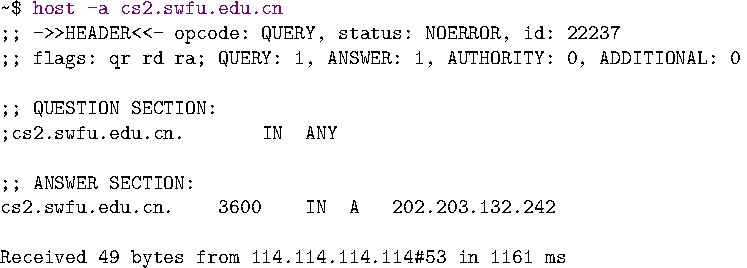
\includegraphics[width=.7\textwidth]{dns-rr-swfu} }
  \end{center}
\end{frame}

\begin{frame}{tcpdump}
  \begin{center}
    \mode<beamer>{ \includegraphics[width=\textwidth]{tcpdump-dns} }%
    \mode<article>{ \includegraphics[width=.7\textwidth]{tcpdump-dns} }
  \end{center}
\end{frame}

See also: \citetitle[Sec.~14.4, \emph{A Simple Example}, p196]{fall2011tcp}

  % \begin{frame}
  %   \begin{iblock}{Resolver}
  %     \begin{itemize}
  %     \item The resolver does not exist as a distinct process running
  %       on the computer.
  %     \item Rather, the resolver is a library of software routines\footnote{\$ man getaddrinfo}
  %       (called the ``resolver code'') that is linked into any program
  %       that needs to look up addresses.
  %     \item This library knows how to ask the name server for host
  %       information.
  %     \end{itemize}
  %   \end{iblock}
  %   \begin{description}
  %   \item[Resolve-only system:] Under BIND, all computers use resolver
  %     code, but not all computers run the name server process. A
  %     computer that does not run a local name server process and
  %     relies on other systems for all name service answers is called a
  %     \emph{resolver-only system}.
  %   \end{description}
  % \end{frame}


% \begin{frame}{BIND}
%   The implementation of DNS used on most UNIX systems is the \emph{Berkeley Internet Name
%     Domain (BIND)} software.
%   \begin{itemize}
%   \item The BIND name server runs as a distinct process called \emph{named} (pronounced
%     "name" "d").
%   \item Name servers are classified differently depending on how they are configured.
%   \end{itemize}

%   How To Configure BIND?
%     \begin{refsection}
%       \nocite{bautts2005linux}
%     \end{refsection}
%     \printbibliography[heading=subbibliography]
% \end{frame}

  % \begin{frame}
  %   \begin{iblock}{Network Information Service, NIS, Yellow Pages}
  %     \begin{itemize}
  %     \item for distributing system configuration data such as user
  %       and host names between computers on a network.
  %     \item an administrative database system developed by Sun
  %       Microsystems.
  %     \end{itemize}
  %   \end{iblock}
  %   \begin{itemize}
  %   \item It provides central control and automatic dissemination of
  %     important administrative files.
  %   \item NIS is mostly used to let several machines in a network
  %     share the same account information (eg the password file).
  %   \item NIS can be used in conjunction with DNS, or as an
  %     alternative to it.
  %   \item NIS + NFS
  %   \end{itemize}
  % \end{frame}

  % \begin{frame}
  %   \begin{iblock}{NIS and DNS have similarities and differences.}
  %     \begin{itemize}
  %     \item Like DNS, NIS overcomes the problem of accurately distributing the host table.
  %     \item Unlike DNS, it provides service only for local area networks.
  %     \item Another difference is that NIS provides access to a wider
  %       range of information than DNS - much more than name-to-address
  %       conversions.
  %       \begin{itemize}
  %       \item It converts several standard UNIX files (e.g.
  %         /etc/hosts, /etc/networks) into databases that can be queried
  %         over the network.  These databases are called \emph{NIS
  %           maps}.
  %       \item The maps can be stored on a central server where they
  %         can be centrally maintained while still being fully
  %         accessible to the NIS clients.
  %       \end{itemize}
  %     \end{itemize}
  %   \end{iblock}
  % \end{frame}

\begin{frame}{DNS References}
  \begin{refsection}
    \nocite{wiki:dns, rfc1034, rfc1035}
    \printbibliography[heading=none]
  \end{refsection}
\end{frame}

%\mode<article>{\clearpage}
\subsection{Mail}

\begin{frame}{E-mail Protocols}
  \begin{iblock}{Proprietary protocols:}
    \begin{description}
    \item[Microsoft:] Outlook client $\Longleftrightarrow$ Exchange server
    \item[IBM:] Notes client $\Longleftrightarrow$ Domino server
    \end{description}
  \end{iblock}
  \begin{iblock}{Open standards:}
    \begin{description}
    \item[SMTP:] Simple Mail Transfer Protocol, RFC2821
    \item[POP3:] Post Office Protocol, RFC1939
    \item[MIME:] Multipurpose Internet Mail Extensions, RFC2045, RFC2046, RFC2047,
      RFC2048, RFC2049
    \item[IMAP4:] Interactive Mail Access Protocol, RFC3501
    \end{description}
  \end{iblock}
\end{frame}
  
\subsubsection{SMTP}

\begin{frame}{SMTP Transports A Mail Object}
  \begin{iblock}{A Mail Object}
    \centering
    \mode<beamer>{ \includegraphics[width=.78\textwidth]{mail_obj} }%
    \mode<article>{ \includegraphics[width=.4\textwidth]{mail_obj} }
    \label{fig:mail_obj}
  \end{iblock}  
\end{frame}

\begin{frame}{A Physical Mail}
  \centering
  \mode<beamer>{ \fbox{\includegraphics[height=.9\textheight]{mail-letter}} }%
  \mode<article>{ \fbox{\includegraphics[width=.3\textwidth]{mail-letter}} }
  \label{fig:letter}
\end{frame}

\begin{frame}%{SMTP}
  \begin{iblock}{The SMTP Basic Structure}
    \begin{center}
      \mode<beamer>{ 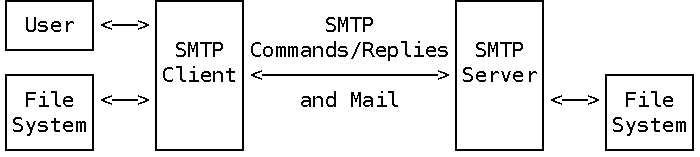
\includegraphics[width=\textwidth]{smtp_model} }%
      \mode<article>{ 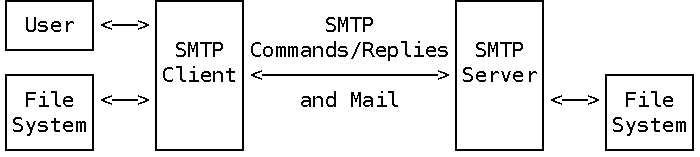
\includegraphics[width=.5\textwidth]{smtp_model} }
    \end{center}
    \label{fig:smtp_model}
  \end{iblock}
  \begin{itemize}
  \item TCP, port 25
  \end{itemize}
\end{frame}

\begin{frame}{Unix File System}
  \centering
  \mode<beamer>{ 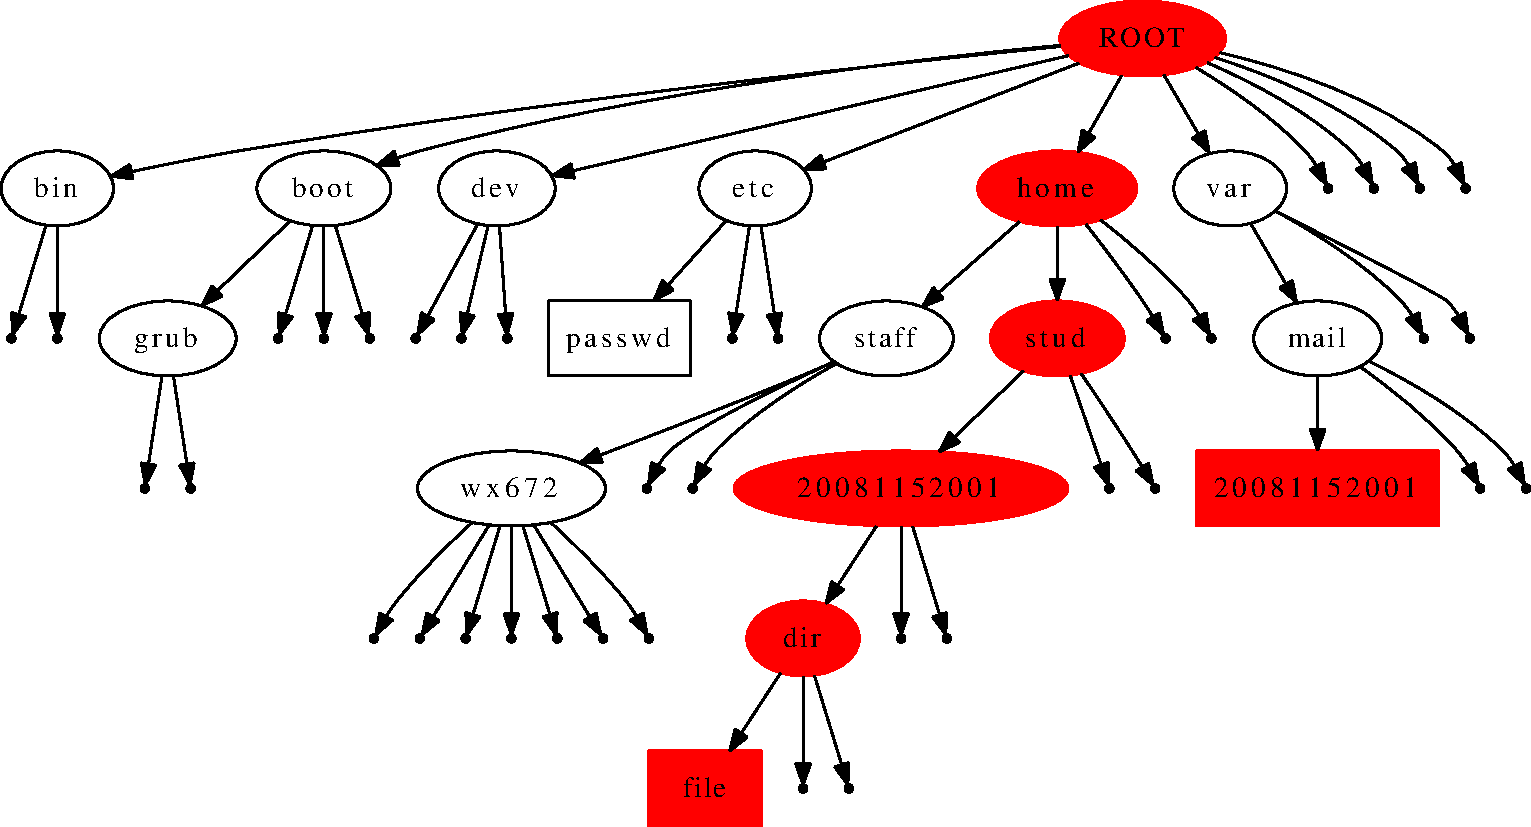
\includegraphics[height=.9\textheight]{cs3} }%
  \mode<article>{ 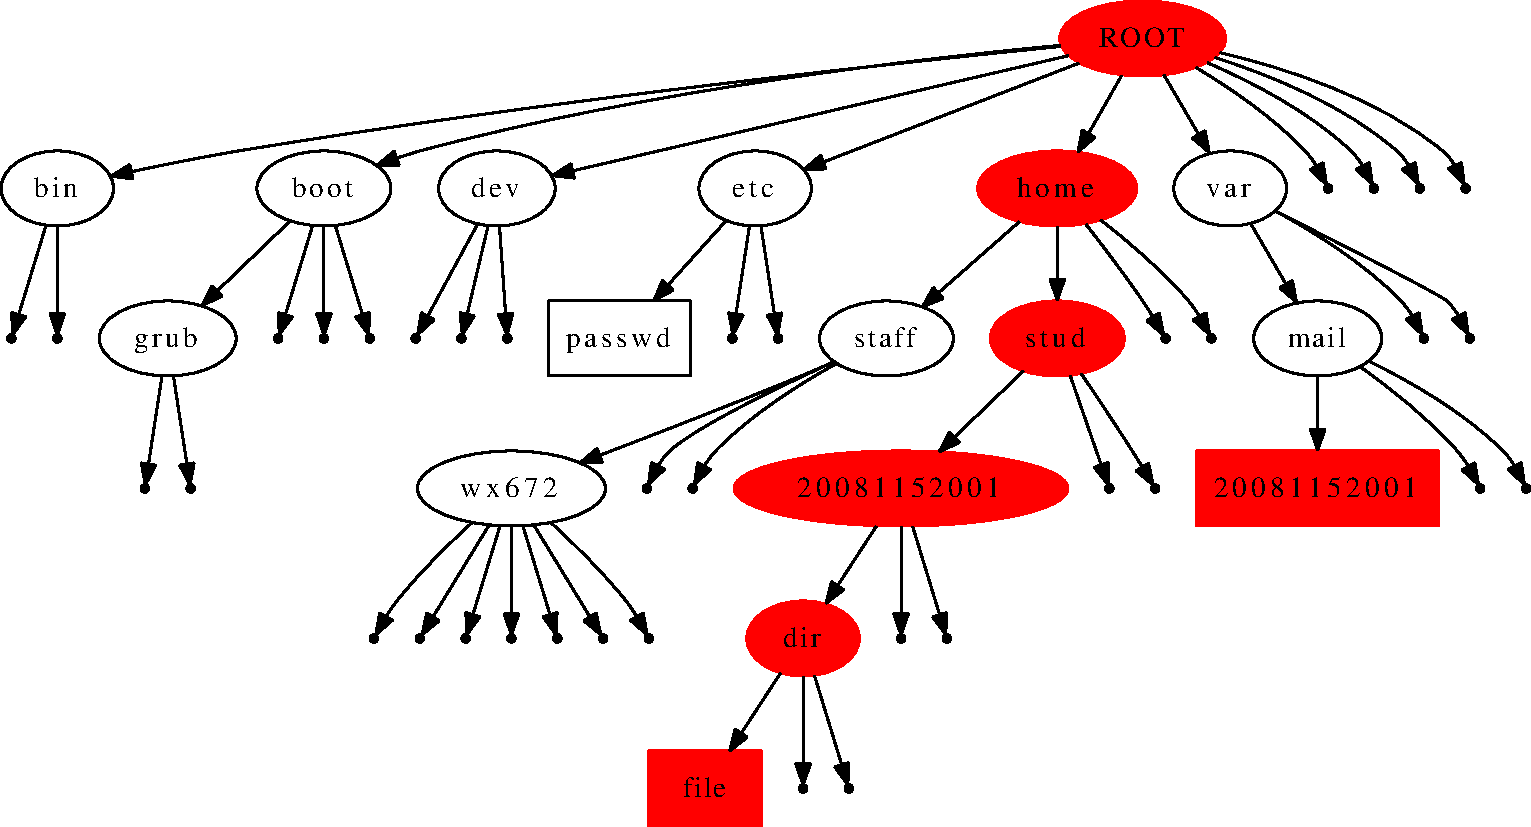
\includegraphics[width=.7\textwidth]{cs3} }
  \label{fig:cs3}
\end{frame}

\begin{frame}%{SMTP Commands}
  \begin{iblock}{SMTP Commands}
    \begin{center}
      \mode<beamer>{ 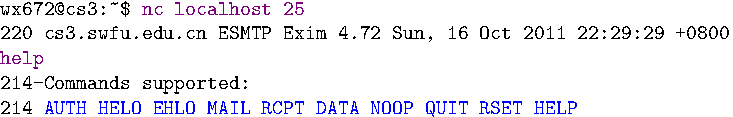
\includegraphics[width=\textwidth]{smtp_cmds} }%
      \mode<article>{ 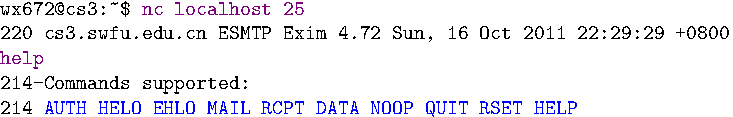
\includegraphics[width=.6\textwidth]{smtp_cmds} }
    \end{center}
  \end{iblock}
  \label{fig:smtp_cmds}
  \begin{itemize}
  \item More commands can be available, depending on your SMTP server configuration.
  \end{itemize}
\end{frame}
  
\begin{frame}{A Simple Protocol}{A SMTP Session}
  \centering
  \mode<beamer>{ \includegraphics[height=.85\textheight]{smtp_session} }%
  \mode<article>{ \includegraphics[width=.5\textwidth]{smtp_session} }
  \label{fig:smtp_session}
\end{frame}

\begin{frame}{Webmail}
  \begin{center}
    \mode<beamer>{ 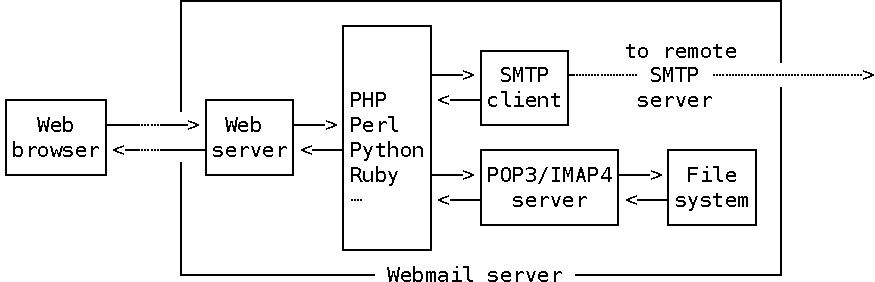
\includegraphics[width=\textwidth]{webmail} }%smtp-pop3
    \mode<article>{ 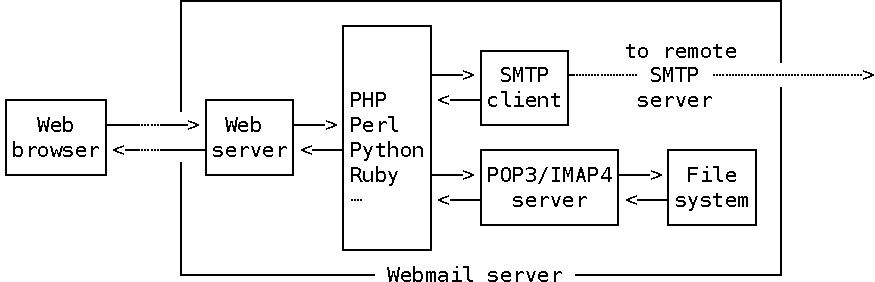
\includegraphics[width=.5\textwidth]{webmail} }%smtp-pop3
  \end{center}
  \label{fig:smtp-pop3}
\end{frame}

\subsubsection{POP3}

\begin{frame}{Post Office Protocol v3}
  \begin{minipage}{.7\linewidth}
    \begin{description}
    \item[POP2] port 109
    \item[POP3] port 110
    \end{description}
    The POP protocols verify the user's login name and password, and move the user's mail
    from the server to the user's local mail reader.
  \end{minipage}\hfill
  \begin{minipage}{.25\linewidth}
    \begin{iblock}{A POP3 Session}
      \centering
      \mode<beamer>{ 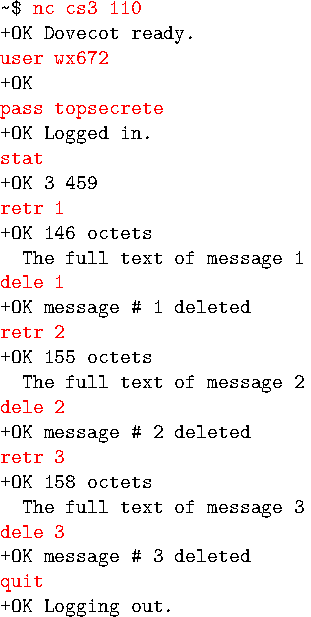
\includegraphics[width=\columnwidth]{pop3_session} }%
      \mode<article>{ 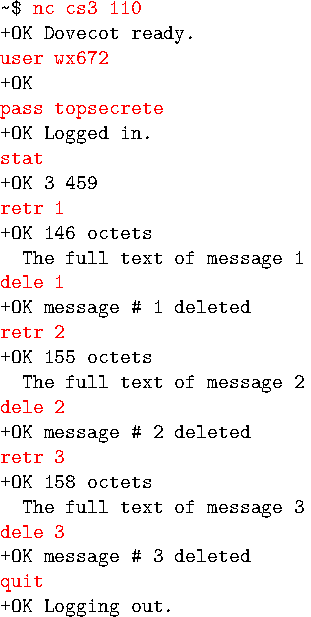
\includegraphics[width=1.5\columnwidth]{pop3_session} }
      \label{fig:pop3_session}
    \end{iblock}
  \end{minipage}
\end{frame}
  
\subsubsection{IMAP}

\begin{frame}{IMAP --- Internet Message Access Protocol}
  \begin{itemize}
  \item port 143
  \end{itemize}
  \begin{iblock}{Advantages over POP3}
    \begin{itemize}
    \item Both connected and disconnected modes of operation
    \item Multiple clients can simultaneously connect to the same mailbox
    \item Access to MIME parts of messages and partial fetch
    \item Message state information kept on the server
    \item Multiple mailboxes on the server
    \item Server-side searches
    \item A built-in extension mechanism
    \end{itemize}
  \end{iblock}
\end{frame}

\begin{frame}{An IMAP session}
  \centering
  \mode<beamer>{ \includegraphics[height=.9\textheight]{imap_session} }%
  \mode<article>{ \includegraphics[width=.6\textwidth]{imap_session} }
\end{frame}
  
\begin{frame}
  \begin{iblock}{Disadvantages of IMAP}
    \begin{itemize}
    \item IMAP is a very heavy and complicated protocol
    \item IMAP generally results in higher server loads than POP3
    \item Server-side searches can potentially use lots of server resources when searching
      massive mailboxes
    \end{itemize}
  \end{iblock}
\end{frame}

\subsubsection{MIME}

\begin{frame}{Multipurpose Internet Mail Extensions}
  \begin{itemize}
  \item SMTP supports only 7-bit ASCII characters.
  \item MIME standard defines mechanisms for emailing other kinds of information, e.g.
    \begin{itemize}
    \item text in languages other than English,
    \item files containing images, sounds, movies,
    \item computer programs
    \end{itemize}
  \item HTTP/MIME
  \end{itemize}
\end{frame}

\begin{frame}{A Typical Mail Header}
  \centering
  \mode<beamer>{ \includegraphics[height=.9\textheight]{mail_header} }%
  \mode<article>{ \includegraphics[width=.6\textwidth]{mail_header} }
  \label{fig:mail_header}
\end{frame}

\subsubsection{Spam}

\begin{frame}{\mode<beamer>{Spam}}
  \begin{itemize}
  \item Any kind of un-wanted email messages
  \item The action of sending such kinds of messages to usenet newsgroups, mailing lists,
    or any other individuals
  \item by year 2000, 7\% of Internet mails were spam
  \item by year 2004, 60\% were spam
  \item Bill Gates receives nearly 4 million emails a day --- mostly spams
  \end{itemize}
\end{frame}

\begin{frame}{How Spam Works?}
  \begin{enumerate}
  \item Collecting Email Addresses (Sniffing, Web Registration, Mailing List and
    Newsgroup, etc.)
  \item Open Relay --- A SMTP server configured in such a way that it allows anyone on
    the Internet to relay (i.e. send) email through it.
  \item Open Proxy --- A proxy which is misconfigured to allow access to anyone on the
    internet.
  \end{enumerate}
\end{frame}

\begin{frame}{Relayed Mail Scenario}
  \centering
  \mode<beamer>{ \includegraphics[height=.9\textheight]{smtp-relay} }%
  \mode<article>{ \includegraphics[width=.5\textwidth]{smtp-relay} }
  \label{fig:relay}
\end{frame}

%  \begin{frame}
%    \begin{figure}
%      \centering
%      \includegraphics[width=\textwidth]{proxy}
%      \caption{ Access To A Server Without Open Proxy}
%      \label{fig:proxy}
%    \end{figure}
%  \end{frame}

\begin{frame}{Common Technologies Of Anti-Spams}
  \begin{itemize}
  \item DNSBL --- DNS-based Blackhole List
  \item Bayesian Filtering: $$P(spam|words) = \frac{P(words|spam)P(spam)}{P(words)}$$
  \item Greylisting --- "normal" MTAs should attempt retries if given an appropriate
    temporary failure code for a delivery attempt.
  \end{itemize}
\end{frame}

\begin{frame}[allowframebreaks]{Mail References}
  \begin{refsection}
    \nocite{wiki:smtp, wiki:pop, wiki:imap, wiki:mime, rfc2821, rfc1939,
      rfc3501, rfc2045}
    \printbibliography[heading=none]
  \end{refsection}
\end{frame}

%\mode<article>{\clearpage}
\subsection{FTP}
  
\begin{frame}\mode<beamer>{FTP}
  \centering
  \mode<beamer>{ \includegraphics[height=.7\textheight]{ftp-model} }%
  \mode<article>{ \includegraphics[width=.5\textwidth]{ftp-model} }
  \label{fig:model}
\end{frame}

\begin{frame}{An Active FTP Session}
  \begin{minipage}{.4\linewidth}
    \begin{description}
    \item[Control session:] $\longrightarrow$
    \end{description}
    \begin{iblock}{To see FTP data session:}
      {\ttfamily\small cs3:\$\quad\textcolor{violet}{nc -l \$((100*256+0))}}
    \end{iblock}
  \end{minipage}\hfill
  \begin{minipage}{.6\linewidth}
    \includegraphics[width=\textwidth]{ftp-actv-ctl}
  \end{minipage}
\end{frame}

% \texttt{PORT h1,h2,h3,h4,p1,p2}
% \begin{itemize}
% \item where \texttt{h1} is the high order 8 bits of the internet host address.
% \end{itemize}
            
\begin{frame}{A Passive FTP Session}
  \begin{minipage}{.4\linewidth}
    \begin{description}
    \item[Control session:] $\longrightarrow$
    \end{description}
    \begin{iblock}{To see FTP data session:}
      {\ttfamily\small cs3:\$}\quad\textcolor{violet}{\texttt{nc cs2 \$((36*256+5))}}
    \end{iblock}
  \end{minipage}\hfill
  \begin{minipage}{.6\linewidth}
    \includegraphics[width=\textwidth]{ftp-psv-ctl}
  \end{minipage}
\end{frame}

\begin{frame}{Active FTP vs. Passive FTP}
  \begin{description}
  \item[In active mode:] Server initiates data connection to client's data port.
  \item[In passive mode:] Client initiates data connection to random port specified by
    server.
  \end{description}
\end{frame}

\begin{frame}{Why Passive Mode?}{Active mode doesn't work with firewall}
  \centering
  \mode<beamer>{ \includegraphics[height=.8\textheight]{ftp-firewall} }%
  \mode<article>{ \includegraphics[width=.8\textwidth]{ftp-firewall} }
\end{frame}

\begin{frame}{FTP References}
  \begin{refsection}
    \nocite{wiki:ftp, rfc959,rfc1579}
    \printbibliography[heading=none]
  \end{refsection}
\end{frame}

%\mode<article>{\clearpage}
\subsection{Peer-to-Peer Applications}

See also \citetitle[Sec.~2.6.1, \emph{P2P File Distribution}]{kurose2013computer}.
  
\begin{frame}{BitTorrent}
  \centering
  \mode<beamer>{\includegraphics[width=.7\textwidth]{bt-ast} }%
  \mode<article>{ \includegraphics[width=.8\textwidth]{bt-ast} }

  {\footnotesize
    \begin{enumerate}
    \item How does a peer find other peers that have the content it wants to download?
    \item How is content replicated by peers to provide high-speed downloads for everyone?
    \item How do peers encourage each other to upload content to others as well as
      download content for themselves?
    \end{enumerate}}
\end{frame}

\begin{description}
\item[torrent] --- a content description file with two key info:
  \begin{itemize}
  \item the name of the tracker
  \item a list of equal-sized chunks (typically 256KiB). The name of each chunk is given
    as a 160-bit SHA-1 hash of the chunk.
  \end{itemize}
\item[tracker] --- the infrastructure node in a swarm that keeps tracking of the status of
  all peers.
\item[swarm] --- a collection of all peers for a transferred file.
\item[peers] --- download chunks of the file from one another.
\item[seeder] --- the peer who has all the chunks (the whole file).
\item[leecher] --- the peer who takes without giving.
\item[Brief workflow:] \,
  \begin{itemize}
  \item When a peer joins a swarm, it registers itself with the tracker;
  \item A peer periodically informs the tracker that it's still in the swarm;
  \item While a peer downloads chunks, it also uploads chunks to others;
  \item When a new peer joins a swarm, the tracker randomly select some peers (say 50)
    from the swarm, and sends their IP addresses to the new peer;
  \item the new peer makes TCP connections with all these 50 peers. Now they're neighbors;
  \item Neighbors ask periodically each other for the list of chunks they have;
  \item Usually each one has a different list, and according to it, they request for
    chunks they don't have from each other (rarest first);
  \item higher upload rate results in higher download rate. Leechers will be
    \emph{choked}.
  \end{itemize}
\end{description}



\begin{frame}{P2P References}
  \begin{refsection}
    \nocite{wiki:bt,cohen08specification}
    \printbibliography[heading=none]
  \end{refsection}
\end{frame}

\mode<all>
%%% Local Variables:
%%% mode: latex
%%% TeX-master: "net-b"
%%% End:
